\begin{figure}[htbp]
  \centering
    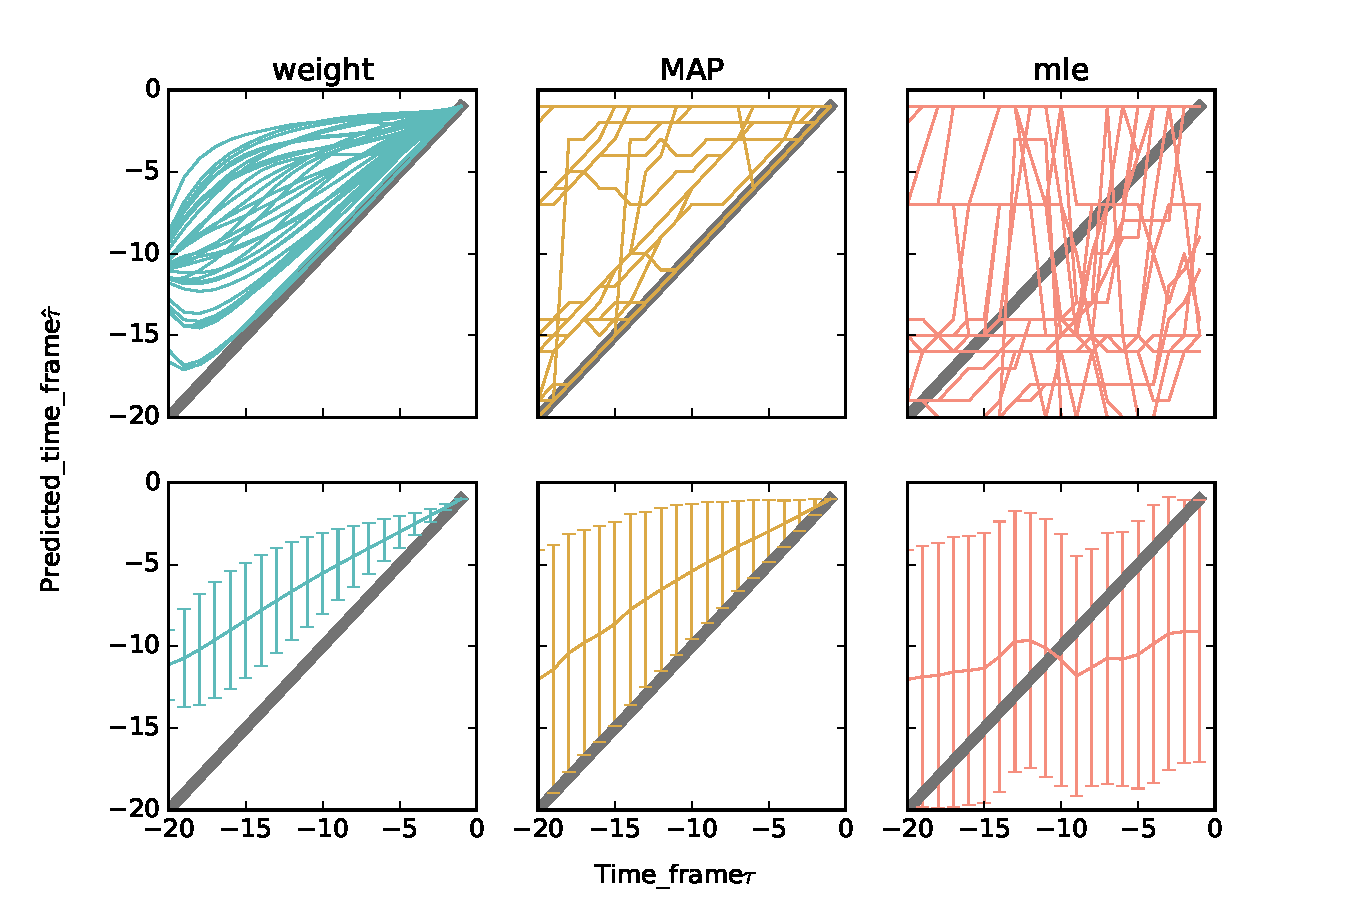
\includegraphics[width=70mm]{fig/result_line_error.pdf}
  \caption{32回の推定結果の推移についての折れ線グラフと,平均,分散をエラーバーで示した図.左から順に,重み付き平均,MAP推定,最尤推定の結果となっている.x軸が実際の時間,y軸が推定時間となっており,実際の時間と推定時間が一致する点を灰色の棒線で繋いでいる.}
  \label{fig:result_line_error}
\end{figure}
